\chapter{Computational Security}\label{Computational-Security}

\paragraph{Additional reading:} Sections 2.3 and 2.4 in Boneh-Shoup
book. Chapter 3 up to and including Section 3.3 in Katz-Lindell book.

Recall our cast of characters- Alice and Bob want to communicate
securely over a channel that is monitored by the nosy Eve. In the last
lecture, we have seen the definition of \emph{perfect secrecy} that
guarantees that Eve cannot learn \emph{anything} about their
communication beyond what she already knew. However, this security came
at a price. For every bit of communication, Alice and Bob have to
exchange in advance a bit of a secret key. In fact, the proof of this
result gives rise to the following simple Python program that can break
every encryption scheme that uses, say, a \(128\) bit key, with a
\(129\) bit message:

\begin{code}
from itertools import product # Import an iterator for cartesian products

# Gets ciphertext as input and two potential plaintexts
# Positive return value means first is more likely,
# negative means second is more likely,
# 0 means both have same likelihood.
#
# We assume we have access to the function Decrypt(key,ciphertext)
def Distinguish(ciphertext,plaintext1,plaintext2):
    bias = 0
    for key in product([0,1], repeat = 128): # Iterate over all possible keys of lenght 128
        p = Decrypt(key, ciphertext)
        if p == plaintext1: bias += 1
        if p == plaintext2: bias -= 1
    return bias
\end{code}

Now, generating, distributing, and protecting huge keys causes immense
logistical problems, which is why almost all encryption schemes used in
practice do in fact utilize short keys (e.g., \(128\) bits long) with
messages that can be much longer (sometimes even terabytes or more of
data).

So, why can't we use the above Python program to break all encryptions
in the Internet and win infamy and fortune? We can in fact, but we'll
have to wait a \emph{really} long time, since the loop in
\texttt{Distinguish} will run \(2^{128}\) times, which will take much
more than the lifetime of the universe to complete, even if we used all
the computers on the planet.

However, the fact that \emph{this} particular program is not a feasible
attack, does not mean there does not exist a different attack. But this
still suggests a tantalizing possibility: if we consider a relaxed
version of perfect secrecy that restricts Eve to performing computations
that can be done in this universe (e.g., less than \(2^{256}\) steps
should be safe not just for human but for all potential alien
civilizations) then can we bypass the impossibility result and allow the
key to be much shorter than the message?

This in fact does seem to be the case, but as we've seen, defining
security is a subtle task, and will take some care. As before, the way
we avoid (at least some of) the pitfalls of so many cryptosystems in
history is that we insist on very precisely \emph{defining} what it
means for a scheme to be secure.

Let us defer the discussion how one defines a function being computable
in ``less than \(T\) operations'' and just say that there is a way to
formally do so. We will want to say that a scheme has ``\(256\) bits of
security'' if it is not possible to break it using less than \(2^{256}\)
operations, and more generally that it has \(t\) bits of security if it
can't be broken using less than \(2^t\) operations. Given the perfect
secrecy definition we saw last time, a natural attempt for defining
Computational secrecy would be the following:

\hypertarget{firstcompdef}{}
\begin{definition}[Computational secrecy (first attempt)] \label[definition]{firstcompdef}

An encryption scheme \((E,D)\) has \emph{\(t\) bits of computational
secrecy} if for every two distinct plaintexts
\(\{m_0,m_1\} \subseteq {\{0,1\}}^\ell\) and every strategy of Eve using
at most \(2^t\) computational steps, if we choose at random
\(b\in{\{0,1\}}\) and a random key \(k\in{\{0,1\}}^n\), then the
probability that Eve guesses \(m_b\) after seeing \(E_k(m_b)\) is at
most \(1/2\).

\end{definition}

\paragraph{Note:} It is important to keep track of what is known and
unknown to the adversary Eve. The adversary knows the set
\(\{ m_0,m_1 \}\) of potential messages, and the ciphertext
\(y=E_k(m_b)\). The only things she doesn't know are whether \(b=0\) or
\(b=1\), and the value of the secret key \(k\). In particular, because
\(m_0\) and \(m_1\) are known to Eve, it does not matter whether we
define Eve's goal in this ``security game'' as outputting \(m_b\) or as
outputting \(b\).

\cref{firstcompdef} seems very natural, but is in fact \emph{impossible}
to achieve if the key is shorter than the message.

\begin{pause} \label[pause]{Before-reading-further-yo}

Before reading further, you might want to stop and think if you can
\emph{prove} that there is no, say, \(\sqrt{n}\) secure encryption
scheme satisfying \cref{firstcompdef} with \(\ell = n+1\) and where the
time to compute the encryption is polynomial.

\end{pause}

The reason \cref{firstcompdef} can't be achieved that if the message is
even one bit longer than the key, we can always have a very efficient
procedure that achieves success probability of about \(1/2 + 2^{-n-1}\)
by guessing the key. That is, we can replace the loop in the Python
program \texttt{Distinguish} by choosing the key at random. Since we
have some small chance of guessing correctly, we will get a small
advantage over half.

Of course an advantage of \(2^{-256}\) in guessing the message is not
really something we would worry about. For example, since the earth is
about 5 billion years old, we can estimate the chance that an asteroid
of the magnitude that caused the dinosaurs' extinction will hit us this
very second to be about \(2^{-60}\). Hence we want to relax the notion
of computational security so it would not consider guessing with such a
tiny advantage as a ``true break'' of the scheme. The resulting
definition is the following:

\hypertarget{compsecconcdef}{}
\begin{definition}[Computational secrecy (concrete)] \label[definition]{compsecconcdef}

An encryption scheme \((E,D)\) has \emph{\(t\) bits of computational
secrecy\footnote{Another version of ``\(t\) bits of security'' is that a
  scheme has \(t\) bits of security if for every \(t_1+t_2 \leq t\), an
  attacker running in \(2^{t_1}\) time can't get success probability
  advantage more than \(2^{-t_2}\). However these two definitions only
  differ from one another by at most a factor of two. This may be
  important for practical applications (where the difference between
  \(64\) and \(32\) bits of security could be crucial) but won't matter
  for our concerns.}} if for every two distinct plaintexts
\(\{m_0,m_1\} \subseteq {\{0,1\}}^\ell\) and every strategy of Eve using
at most \(2^t\) computational steps, if we choose at random
\(b\in{\{0,1\}}\) and a random key \(k\in{\{0,1\}}^n\), then the
probability that Eve guesses \(m_b\) after seeing \(E_k(m_b)\) is at
most \(1/2+2^{-t}\).

\end{definition}

Having learned our lesson, let's try to see that this strategy does give
us the kind of conditions we desired. In particular, let's verify that
this definition implies the analogous condition to perfect secrecy.

\hypertarget{twotomanycomp}{}
\begin{theorem}[Guessing game for computational secrecy] \label[theorem]{twotomanycomp}

If \((E,D)\) is has \(t\) bits of Computational secrecy as per
\cref{compsecconcdef} then every subset \(M \subseteq {\{0,1\}}^\ell\)
and every strategy of Eve using at most \(2^t-(100\ell+100)\)
computational steps, if we choose at random \(m\in M\) and a random key
\(k\in{\{0,1\}}^n\), then the probability that Eve guesses \(m\) after
seeing \(E_k(m_b)\) is at most \(1/|M|+2^{-t+1}\).

\end{theorem}

Before proving this theorem note that it gives us a pretty strong
guarantee. In the exercises we will strengthen it even further showing
that no matter what prior information Eve had on the message before, she
will never get any non-negligible new information on it. One way to
phrase it is that if the sender used a \(256\)-bit secure encryption to
encrypt a message, then your chances of getting to learn any additional
information about it before the universe collapses are more or less the
same as the chances that a fairy will materialize and whisper it in your
ear.

\begin{pause} \label[pause]{Before-reading-the-proof-}

Before reading the proof, try to again review the proof of
\cref{twotomanythm}, and see if you can generalize it yourself to the
computational setting.

\end{pause}

\begin{proof}[Proof of \cref{twotomanycomp}] \label[proof]{The-proof-is-rather-simil}

The proof is rather similar to the equivalence of guessing one of two
messages vs.~one of many messages for perfect secrecy (i.e.,
\cref{twotomanythm}). However, in the computational context we need to
be careful in keeping track of Eve's running time. In the proof of
\cref{twotomanythm} we showed that if there exists:

\begin{itemize}
\tightlist
\item
  A subset \(M\subseteq {\{0,1\}}^\ell\) of messages
\end{itemize}

and

\begin{itemize}
\tightlist
\item
  An adversary \(Eve:{\{0,1\}}^o\rightarrow{\{0,1\}}^\ell\) such that
\end{itemize}

\[
\Pr_{m{\leftarrow_{\tiny R}}M, k{\leftarrow_{\tiny R}}{\{0,1\}}^n}[ Eve(E_k(m))=m ] > 1/|M|
\]

Then there exist two messages \(m_0,m_1\) and an adversary
\(Eve':{\{0,1\}}^0\rightarrow{\{0,1\}}^\ell\) such that
\(\Pr_{b{\leftarrow_{\tiny R}}{\{0,1\}},k{\leftarrow_{\tiny R}}{\{0,1\}}^n}[Eve'(E_k(m_b))=m_b ] > 1/2\).

To adapt this proof to the computational setting and complete the proof
of the current theorem it suffices to show that:

\begin{itemize}
\item
  If the probability of \(Eve\) succeeding was
  \(\tfrac{1}{|M|} + \epsilon\) then the probability of \(Eve'\)
  succeeding is at least \(\tfrac{1}{2} + \epsilon/2\).
\item
  If \(Eve\) can be computed in \(T\) operations, then \(Eve'\) can be
  computed in \(T + 100\ell + 100\) operations.
\end{itemize}

This will imply that if \(Eve\) ran in polynomial time and had
polynomial advantage over \(1/|M|\) in guessing a plaintext chosen from
\(M\), then \(Eve'\) would run in polynomial time and have polynomial
advantage over \(1/2\) in guessing a plaintext chosen from
\(\{ m_0,m_1\}\).

The first item can be shown by simply doing the same proof more
carefully, keeping track how the advantage over \(\tfrac{1}{|M|}\) for
\(Eve\) translates into an advantage over \(\tfrac{1}{2}\) for \(Eve'\).
As the world's most annoying saying goes, doing this is an excellent
exercise for the reader. The item point is obtained by looking at the
definition of \(Eve'\) from that proof. On input \(c\), \(Eve'\)
computed \(m=Eve(c)\) (which costs \(T\) operations), checked if
\(m=m_0\) (which costs, say, at most \(5\ell\) operations), and then
outputted either \(1\) or a random bit (which is a constant, say at most
\(100\) operations).

\end{proof}

\subsection{Proof by reduction}\label{Proof-by-reduction}

The proof of \cref{twotomanycomp} is a model to how a great many of the
results in this course will look like. Generally we will have many
theorems of the form:

\begin{quote}
``If there is a scheme \(S'\) satisfying security definition \(X'\) then
there is a scheme \(S\) satisfying security definition \(X\)''
\end{quote}

In the context of \cref{twotomanycomp}, \(X'\) was ``having \(t\) bits
of security'' (in the context distinguishing between encryptions of two
ciphertexts) and \(X\) was the more general notion of hardness of
getting a non-trivial advantage over guessing for an encryption of a
random \(m\in M\). While in \cref{twotomanycomp} the encryption scheme
\(S\) was the same as \(S'\), this need not always be the case. However,
all of the proofs of such statements will have the same global
structure--- we will assume towards a contradiction, that there is an
efficient adversary strategy \(Eve\) demonstrating that the scheme \(S\)
violates the security notion \(X\), and build from \(Eve\) a strategy
\(Eve'\) demonstrating that \(S'\) violates \(X\). This is such an
important point that it deserves repeating:

\begin{quote}
\emph{The way you show that if \(S'\) is secure then \(S\) is secure is
by giving a transformation from an adversary that breaks \(S\) into an
adversary that breaks \(S'\)}
\end{quote}

For computational secrecy, we will always want that \(Eve'\) will be
efficient if \(Eve\) is, and that will usually be the case because
\(Eve'\) will simply use \(Eve\) as a black box, which it will not
invoke too many times, and addition will use some polynomial time
preprocessing and postprocessing. The more challenging parts of such
proofs are typically:

\begin{itemize}
\item
  Coming up with the strategy \(Eve'\).
\item
  Analyzing the probability of success and in particular showing that if
  \(Eve\) had non-negligible advantage then so will \(Eve'\).
\end{itemize}


\begin{marginfigure}
\centering
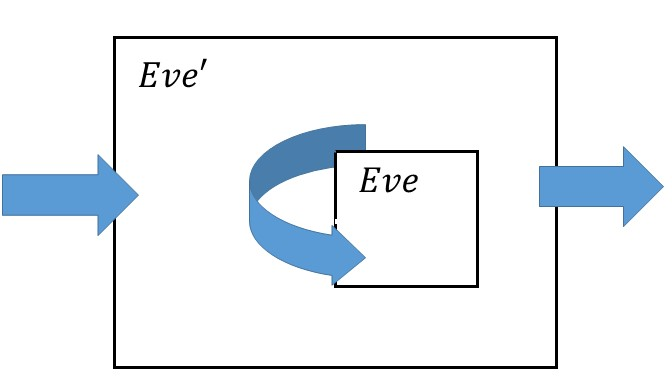
\includegraphics[width=\linewidth, height=1.5in, keepaspectratio]{../figure/reduction.jpg}
\caption{We show that the security of \(S'\) implies the security of
\(S\) by transforming an adversary \(Eve\) breaking \(S\) into an
adversary \(Eve'\) breaking \(S'\).}
\label{reductiongenfig}
\end{marginfigure}

Note that, just like in the context of NP completeness or
uncomputability reductions, security reductions work \emph{backwards}.
That is, we construct the scheme \(S\) based on the scheme \(S'\), but
then prove that we can transform an algorithm breaking \(S\) into an
algorithm breaking \(S'\). Just like in computational complexity, it can
sometimes be hard to keep track of the direction of the reduction. In
fact, cryptographic reductions can be even subtler, since they involve
an interplay of several entities (for example, sender, receiver, and
adversary) and probabilistic choices (e.g., over the message to be sent
and the key).

\section{The asymptotic approach}\label{The-asymptotic-approach}

For practical security, often every bit of security matters. We want our
keys to be as short as possible and our schemes to be as fast as
possible while satisfying a particular level of security. In practice we
would usually like to ensure that when we use a smallish security
parameter such as \(n\) in the few hundreds or thousands then:

\begin{itemize}
\item
  The \emph{honest parties} (the parties running the encryption and
  decryption algorithms) are extremely efficient, something like
  100-1000 cycles per byte of data processed. In theory terms we would
  want them be using an \(O(n)\) or at worst \(O(n^2)\) time algorithms
  with not-too-big hidden constants.
\item
  We want to protect against \emph{adversaries} (the parties trying to
  break the encryption) that have much vaster computational
  capabilities. A typical modern encryption is built so that using
  standard key sizes it can withstand the combined computational powers
  of all computers on earth for several decades. In theory terms we
  would want the time to break the scheme be at least \(2^{\Omega(n)}\)
  or \(2^(\Omega(\sqrt{n})\) / \(2^{\Omega(n^{1/3})}\) with not too
  small hidden constants.
\end{itemize}

For understanding the \emph{principles} behind cryptography, keeping
track of those bits can be a distraction, and so just like we do in
algorithms courses, we will use \emph{asymptotic analysis} (also known
as \emph{big Oh notation}) to sweep many of those details under the
carpet.

To a first approximation, there will be only two types of running times
we will encounter in this course:

\begin{itemize}
\item
  \emph{Polynomial} running time of the form \(d\cdot n^c\) for some
  constants \(d,c>0\) (or \(poly(n)=n^{O(1)}\) for short) , which we
  will consider as \emph{efficient}
\item
  \emph{Exponential} running time of the form
  \(2^{d\cdot n^{\epsilon}}\) for some constants \(d,\epsilon >0\) (or
  \(2^{n^{\Omega(1)}}\) for short) which we will consider as
  \emph{infeasible}.\footnote{Some texts reserve the term
    \emph{exponential} to functions of the form \(2^{\epsilon n}\) for
    some \(\epsilon > 0\) and call a function such as, say,
    \(2^{\sqrt{n}}\) \emph{subexponential} . However, we will generally
    not make this distinction in this course.}
\end{itemize}

Another way to say it is that in this course, if a scheme has any
security at all, it will have at least \(n^{\epsilon}\) bits of security
where \(n\) is the length of the key and \(\epsilon>0\) is some absolute
constant such as \(\epsilon=1/3\).

These are not all the theoretically possible running times. One can have
intermediate functions such as \(n^{\log n}\) though we will generally
not encounter those. To make things clean (and to correspond to standard
terminology), we will say that an algorithm \(A\) is \emph{efficient} if
it runs in time \(poly(n)\) when \(n\) is its input length (which will
always be the same, up to polynomial factors, as the key length). If
\(\mu(n)\) is some probability that depends on the input/key length
parameter \(n\), then we say that \(\mu(n)\) is \emph{negligible} if
it's smaller than every polynomial. That is, we make the following
definition

\hypertarget{negligibledef}{}
\begin{definition}[Negligible function] \label[definition]{negligibledef}

A function \(\mu:\mathbb{N} \rightarrow [0,\infty)\) is
\emph{negligible} if for every polynomial \(p:\N \rightarrow \N\) there
exists \(N \in \N\) such that \(\mu(n) < \tfrac{1}{p(n)}\) for every
\(n>N\).\^{}{[}Negligible functions are sometimes defined with image
equalling \([0,1]\) as opposed to the set \([0,\infty)\) of non-negative
real numbers, since they are typically used to bound probabilities.
However, this does not make much difference since if \(\mu\) is
negligible then for large enough \(N\), \(\mu(n)\) will be smaller than
one. {]}

\end{definition}

The following exercises are good ways to get some comfort with this
definition

\hypertarget{negligible}{}
\begin{exercise}[Negligible functions properties] \label[exercise]{negligible}

\begin{enumerate}
\def\labelenumi{\arabic{enumi}.}
\item
  Let \(\mu:\N \rightarrow [0,\infty)\) be a negligible function. Prove
  that for every polynomials \(p,q:\R \rightarrow \R\) with non-negative
  coefficients, the function \(\mu':\N \rightarrow [0,\infty)\) defined
  as \(\mu'(n) = p(\mu(q(n)))\) is negligible.
\item
  Let \(\mu:\N \rightarrow \R\). Prove that \(\mu\) is negligible if and
  only if for every constant \(c\),
  \(\lim_{n \rightarrow \infty} n^c \mu(n) = 0\).
\end{enumerate}

\end{exercise}

\hypertarget{asymptotic}{}
\begin{remark}[Asymptotic analysis] \label[remark]{asymptotic}

The above definitions could be confusing if you haven't encountered
asymptotic analysis before. Reading the beginning of Chapter 3 (pages
43-51) in the KL book, as well as the mathematical background lecture in
my \href{http://www.introtcs.org/public/index.html}{intro to TCS notes}
can be extremely useful. As a rule of thumb, if every time you see the
word ``polynomial'' you imagine the function \(n^{10}\) and every time
you see the word ``negligible'' you imagine the function
\(2^{-\sqrt{n}}\) then you will get the right intuition.

What you need to remember is that negligible is much smaller than any
inverse polynomial, while polynomials are closed under multiplication,
and so we have the ``equations''

\[negligible\times polynomial = negligible\]

and

\[polynomial \times polynomial = polynomial\]

As mentioned, in practice people really want to get as close as possible
to \(n\) bits of security with an \(n\) bit key, but we would be happy
as long as the security grows with the key, so when we say a scheme is
``secure'' you can think of it having \(\sqrt{n}\) bits of security
(though any function growing faster than \(\log n\) would be fine as
well).

\end{remark}

From now on, we will require all of our encryption schemes to be
\emph{efficient} which means that the encryption and decryption
algorithms should run in polynomial time. Security will mean that any
efficient adversary can make at most a negligible gain in the
probability of guessing the message over its a priori
probability.\footnote{Note that there is a subtle issue here with the
  order of quantifiers. For a scheme to be efficient, the algorithms
  such as encryption and decryption need to run in some \emph{fixed}
  polynomial time such as \(n^2\) or \(n^3\). In contrast we allow the
  adversary to run in \emph{any} polynomial time. That is, for every
  \(c\), if \(n\) is large enough, then the scheme should be secure
  against an adversary that runs in time \(n^c\). This is in line with
  the general principle in cryptography that we always allow the
  adversary potentially much more resources than those used by the
  honest users. In practical security we often assume that the gap
  between the honest use and the adversary resources can be
  \emph{exponential}. For example, a low power embedded device can
  encrypt messages that, as far as we know, are undecipherable even by a
  nation-state using super-computers and massive data centers.} That is,
we make the following definition:

\hypertarget{compsecdef}{}
\begin{definition}[Computational secrecy (asymptotic)] \label[definition]{compsecdef}

An encryption scheme \((E,D)\) is \emph{computationally secret} if for
every two distinct plaintexts \(\{m_0,m_1\} \subseteq {\{0,1\}}^\ell\)
and every efficient (i.e., polynomial time) strategy of Eve, if we
choose at random \(b\in{\{0,1\}}\) and a random key \(k\in{\{0,1\}}^n\),
then the probability that Eve guesses \(m_b\) after seeing \(E_k(m_b)\)
is at most \(1/2+\mu(n)\) for some negligible function \(\mu(\cdot)\).

\end{definition}

\subsection{Counting number of
operations.}\label{Counting-number-of-operat}

One more detail that we've so far ignored is what does it mean exactly
for a function to be computable using at most \(T\) operations.
Fortunately, when we don't really care about the difference between
\(T\) and, say, \(T^2\), then essentially every reasonable definition
gives the same answer.\footnote{With some caveats that need to be added
  due to \emph{quantum computers}: we'll get to those later in the
  course, though they won't change most of our theory.} Formally, we can
use the notions of Turing machines, Boolean circuits, or straightline
programs to define complexity. For concreteness, lets define that a
function \(F:{\{0,1\}}^n\rightarrow{\{0,1\}}^m\) has complexity at most
\(T\) if there is a Boolean circuit that computes \(F\) using at most
\(T\) Boolean gates (say AND/OR/NOT or NAND, or you can choose your
favorite universal gate sets.) We will often also consider
\emph{probabilistic} functions in which case we allow the circuit a RAND
gate that outputs a single random bit (though this in general does not
give extra power). The fact that we only care about asymptotics means
you don't really need to think of gates, etc.. when arguing in
cryptography. However, it is comforting to know that this notion has a
precise mathematical formulation.

We could also have used Turing Machines. The main reason we use
circuits, which are a non-uniform model, is that:

\begin{enumerate}
\def\labelenumi{\arabic{enumi}.}
\item
  Circuits can express \emph{finite} computation, while Turing machines
  only make sense for computing on arbitrarily large input lengths, and
  so we can make sense of notions such as ``\(t\) bits of computational
  security''.
\item
  Circuits allow the notion of ``hardwiring'' whereby if we can compute
  a certain function \(F:\{0,1\}^{n+s} \rightarrow \{0,1\}^m\) using a
  circuit of \(T\) gates and have a string \(w \in \{0,1\}^s\) then we
  can compute the function \(x \mapsto F(xw)\) using \(T\) gates as
  well. This is useful in many cryptograhic proofs.
\end{enumerate}

One can build the theory of cryptography using Turing machines as well,
but it is more cumbersome.

\paragraph{Computing beyond functions.} Later on in the course, both our
cryptographic schemes and the adversaries will extend beyond simple
functions that map an input to an output, and we will consider
\emph{interactive algorithms} that exchange messages with one another.
Such an algorithm can be implemented using circuits or Turing machines
that take as input the prior state and the history of messages up to a
certain point in the interaction, and output the next message in the
interaction. The number of operations used in such a strategy is the
total number of gates used in computing all the messages.

\section{Our first conjecture}\label{Our-first-conjecture}

We are now ready to make our first conjecture:

\begin{quote}
\textbf{The Cipher Conjecture:}\footnote{As will be the case for other
  conjectures we talk about, the name ``The Cipher Conjecture'' is not a
  standard name, but rather one we'll use in this course. In the
  literature this conjecture is mostly referred to as the conjecture of
  existence of \emph{one way functions}, a notion we will learn about
  later. These two conjectures a priori seem quite different but have
  been shown to be equivalent.} There exists a computationally secret
encryption scheme \((E,D)\) (where \(E,D\) are efficient) with a key of
size \(n\) for messages of size \(n+1\).
\end{quote}

A \emph{conjecture} is a well defined mathematical statement which (1)
we believe is true but (2) don't know yet how to prove. Proving the
cipher conjecture will be a great achievement and would in particular
settle the P vs NP question, which is arguably \emph{the} fundamental
question of computer science. That is, the following theorem is known:

\hypertarget{PNPcipherthm}{}
\begin{theorem}[Breaking crypto if P=NP] \label[theorem]{PNPcipherthm}

If \(P=\ensuremath{\mathit{NP}}\) then there does not exist a
computationally secret encryption with efficient \(E\) and \(D\) and
where the message is longer than the key.

\end{theorem}

\begin{proof} \label[proof]{We-just-sketch-the-proof-}

We just sketch the proof, as this is not the focus of this course. If
\(P=\ensuremath{\mathit{NP}}\) then whenever we have a loop that
searches through some domain to find some string that satisfies a
particular property (like the loop in the \texttt{Distinguish}
subroutine above that searches over all keys) then this loop can be sped
up \emph{exponentially} .

\end{proof}

While it is very widely believed that
\(P\neq \ensuremath{\mathit{NP}}\), at the moment we do not know how to
\emph{prove} this, and so have to settle for accepting the cipher
conjecture as essentially an axiom, though we will see later in this
course that we can show it follows from some seemingly weaker
conjectures.

There are several reasons to believe the cipher conjecture. We now
briefly mention some of them:

\begin{itemize}
\item
  \emph{Intuition:} If the cipher conjecture is false then it means that
  for \emph{every} possible cipher we can make the exponential time
  attack described above become efficient. It seems ``too good to be
  true'' in a similar way that the assumption that P=NP seems too good
  to be true.
\item
  \emph{Concrete candidates:} As we will see in the next lecture, there
  are several concrete candidate ciphers using keys shorter than
  messages for which despite \emph{tons} of effort, no one knows how to
  break them. Some of them are widely used and hence governments and
  other benign or not so benign organizations have every reason to
  invest huge resources in trying to break them. Despite that as far as
  we know (and we know a little more after Edward Snowden's revelations)
  there is no significant break known for the most popular ciphers.
  Moreover, there are other ciphers that can be based on canonical
  mathematical problems such as factoring large integers or decoding
  random linear codes that are immensely interesting in their own right,
  independently of their cryptographic applications.
\item
  \emph{Minimalism:} Clearly if the cipher conjecture is false then we
  also don't have a secure encryption with a key, say, twice as long as
  the message. But it turns out the cipher conjecture is in fact
  \emph{necessary} for essentially every cryptographic primitive,
  including not just private key and public key encryptions but also
  digital signatures, hash functions, pseudorandom generators, and more.
  That is, if the cipher conjecture is false then to a large extent
  cryptography does not exist, and so we essentially have to assume this
  conjecture if we want to do any kind of cryptography.
\end{itemize}

\section{Why care about the cipher
conjecture?}\label{Why-care-about-the-cipher}

\begin{quote}
\emph{``Give me a place to stand, and I shall move the world''}
Archimedes, circa 250 BC
\end{quote}

Every perfectly secure encryption scheme is clearly also computationally
secret, and so if we required a message of size \(n\) instead \(n+1\),
then the conjecture would have been trivially satisfied by the one-time
pad. However, having a message longer than the key by just a single bit
does not seem that impressive. Sure, if we used such a scheme with
\(128\)-bit long keys, our communication will be smaller by a factor of
\(128/129\) (or a saving of about \(0.8\%\)) over the one-time pad, but
this doesn't seem worth the risk of using an unproven conjecture.
However, it turns out that if we assume this rather weak condition, we
can actually get a computationally secret encryption scheme with a
message of size \(p(n)\) for \emph{every} polynomial \(p(\cdot)\). In
essence, we can fix a single \(n\)-bit long key and communicate securely
as many bits as we want!

Moreover, this is just the beginning. There is a huge range of other
useful cryptographic tools that we can obtain from this seemingly
innocent conjecture: (We will see what all these names and some of these
reductions mean later in the course.)


\begin{figure}
\centering
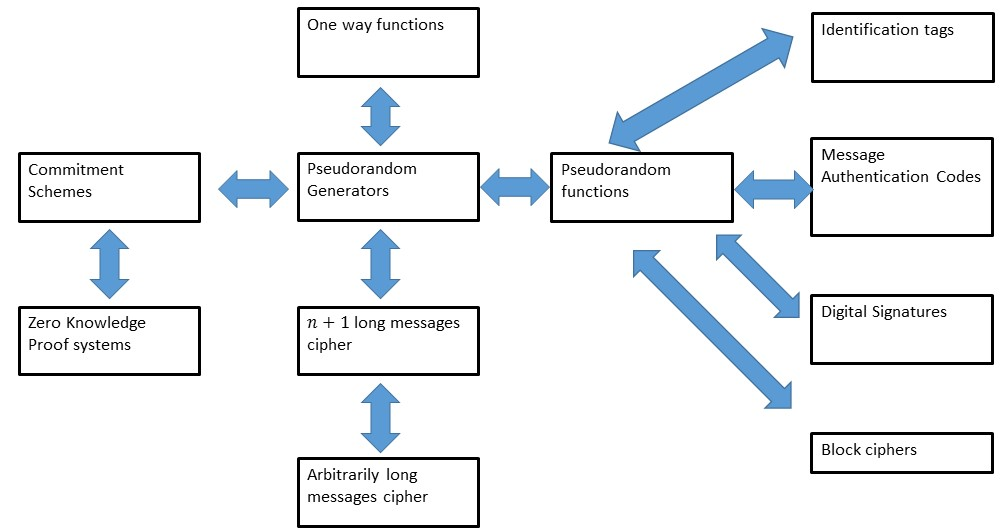
\includegraphics[width=\textwidth, height=0.25\paperheight, keepaspectratio]{../figure/privatekey-reduction-web.jpg}
\caption{Web of reductions between notions equivalent to ciphers with
larger than key messages}
\label{tmplabelfig}
\end{figure}

We will soon see the first of the many reductions we'll learn in this
course. Together this ``web of reductions'' forms the scientific core of
cryptography, connecting many of the core concepts and enabling us to
construct increasingly sophisticated tools based on relatively simple
``axioms'' such as the cipher conjecture.

\section{Prelude: Computational
Indistinguishability}\label{Prelude-Computational-Ind}

The task of Eve in breaking an encryption scheme is to
\emph{distinguish} between an encryption of \(m_0\) and an encryption of
\(m_1\). It turns out to be useful to consider this question of when two
distributions are \emph{computationally indistinguishable} more broadly:

\hypertarget{compindef}{}
\begin{definition}[Computational Indistinguishability] \label[definition]{compindef}

Let \(X\) and \(Y\) be two distributions over \({\{0,1\}}^o\). We say
that \(X\) and \(Y\) are \((T,\epsilon)\)\emph{-computationally
indistinguishable}, denoted by \(X \approx_{T,\epsilon} Y\), if for
every function \(Eve\) computable with at most \(T\) operations,

\[
| \Pr[ Eve(X) = 1 ] - \Pr[ Eve(Y) = 1 ] | \leq \epsilon \;.
\]

We say that \(X\) and \(Y\) are simply \emph{computationally
indistinguishable}, denoted by \(X\approx Y\), if they are
\((T,\epsilon)\) indistinguishable for every polynomial \(T(o)\) and
inverse polynomial \(\epsilon(o)\).\footnote{This definition implicitly
  assumes that \(X\) and \(Y\) are actually \emph{parameterized} by some
  number \(n\) (that is polynomially related to \(o\)) so for every
  polynomial \(T(o)\) and inverse polynomial \(\epsilon(o)\) we can take
  \(n\) to be large enough so that \(X\) and \(Y\) will be
  \((T,\epsilon)\) indistinguishable. In all the cases we will consider,
  the choice of the parameter \(n\) (which is usually the length of the
  key) will be clear from the context.}

\end{definition}

\paragraph{Note:} The expression \(\Pr[ Eve(X)=1]\) can also be written
as \({\mathbb{E}}[Eve(X)]\) (since we can assume that whenever
\(Eve(x)\) does not output \(1\) it outputs zero). This notation will be
useful for us sometimes.

We can use computational indistinguishability to phrase the definition
of Computational secrecy more succinctly:

\hypertarget{compindsecthm}{}
\begin{theorem}[Computational Indistinguishability phrasing of security] \label[theorem]{compindsecthm}

Let \((E,D)\) be a valid encryption scheme. Then \((E,D)\) is
computationally secret if and only if for every two messages
\(m_0,m_1 \in \{0,1\}^\ell\),
\[ \{ E_k(m_0) \}  \approx \{ E_k(m_1) \}  \] where each of these two
distributions is obtained by sampling a random
\(k{\leftarrow_{\tiny R}}{\{0,1\}}^n\).

\end{theorem}

Working out the proof is an excellent way to make sure you understand
both the definition of Computational secrecy and computational
indistinguishability, and hence we leave it as an exercise.

One intuition for computational indistinguishability is that it is
related to some notion of \emph{distance}. If two distributions are
computationally indistinguishable, then we can think of them as ``very
close'' to one another, at least as far as efficient observers are
concerned. Intuitively, if \(X\) is close to \(Y\) and \(Y\) is close to
\(Z\) then \(X\) should be close to \(Z\).\footnote{Results of this form
  are known as ``triangle inequalities'' since they can be viewed as
  generalizations of the statement that for every three points on the
  plane \(x,y,z\), the distance from \(x\) to \(z\) is not larger than
  the distance from \(x\) to \(y\) plus the distance from \(y\) to
  \(z\). In other words, the edge \(\overline{x,z}\) of the triangle
  \((x,y,z)\) is not longer than the sum of the lengths of the other two
  edges \(\overline{x,y}\) and \(\overline{y,z}\).} Similarly if four
distributions \(X,X',Y,Y'\) satisfy that \(X\) is close to \(Y\) and
\(X'\) is close to \(Y'\), then you might expect that the distribution
\((X,X')\) where we take two independent samples from \(X\) and \(X'\)
respectively, is close to the distribution \((Y,Y')\) where we take two
independent samples from \(Y\) and \(Y'\) respectively. We will now
verify that these intuitions are in fact correct:

\hypertarget{triangleeqthm}{}
\begin{theorem}[Triangle Inequality for Computational Indistinguishability] \label[theorem]{triangleeqthm}

Suppose
\(\{ X_1 \} \approx_{T,\epsilon} \{ X_2 \} \approx_{T,\epsilon} \cdots \approx_{T,\epsilon} \{ X_m \}\).
Then \(\{ X_1 \} \approx_{T, (m-1)\epsilon} \{ X_m \}\).

\end{theorem}

\begin{proof} \label[proof]{Suppose-that-there-exists}

Suppose that there exists a \(T\) time \(Eve\) such that \[
|\Pr[ Eve(X_1)=1] - \Pr[ Eve(X_m)=1]| > (m-1)\epsilon  \;.
\]

Write \[
\Pr[ Eve(X_1)=1] - \Pr[ Eve(X_m)=1] = \sum_{i=1}^{m-1} \left( \Pr[ Eve(X_i)=1] - \Pr[ Eve(X_{i+1})=1] \right)  \;.
\]

Thus, \[
\sum_{i=1}^{m-1} \left| \Pr[ Eve(X_i)=1] - \Pr[ Eve(X_{i+1})=1] \right| > (m-1)\epsilon
\] and hence in particular there must exists some
\(i\in\{1,\ldots,m-1\}\) such that \[
\left| \Pr[ Eve(X_i)=1] - \Pr[ Eve(X_{i+1})=1] \right| > \epsilon
\] contradicting the assumption that
\(\{ X_i \} \approx_{T,\epsilon} \{ X_{i+1} \}\) for all
\(i\in\{1,\ldots,m-1\}\).

\end{proof}

\hypertarget{compindrepthm}{}
\begin{theorem}[Computational Indistinguishability is preserved under repetition] \label[theorem]{compindrepthm}

Suppose that \(X_1,\ldots,X_\ell,Y_1,\ldots,Y_\ell\) are distributions
over \({\{0,1\}}^n\) such that \(X_i \approx_{T,\epsilon} Y_i\). Then
\((X_1,\ldots,X_\ell) \approx_{T-10\ell n,\ell\epsilon} (Y_1,\ldots,Y_\ell)\).

\end{theorem}

\begin{proof} \label[proof]{For-every-iinldotsell-we-}

For every \(i\in\{0,\ldots,\ell\}\) we define \(H_i\) to be the
distribution \((X_1,\ldots,X_i,Y_{i+1},\ldots,Y_\ell)\). Clearly
\(H_0 = (X_1,\ldots,X_\ell)\) and \(H_\ell = (Y_1,\ldots,Y_\ell)\). We
will prove that for every \(i\),
\(H_i \approx_{T-10\ell n,\epsilon} H_{i+1}\), and the proof will then
follow from the triangle inequality (can you see why?). Indeed, suppose
towards the sake of contradiction that there was some
\(i\in \{0,\ldots,\ell\}\) and some \(T-10\ell n\)-time
\(Eve's:{\{0,1\}}^{n\ell}\rightarrow{\{0,1\}}\) such that

\[
\left| {\mathbb{E}}[ Eve'(H_i) ] - {\mathbb{E}}[ Eve(H_{i+1}) ] \right|  > \epsilon\;.
\]

In other words \[
\left| {\mathbb{E}}_{X_1,\ldots,X_{i-1},Y_i,\ldots,Y_\ell}[ Eve'(X_1,\ldots,X_{i-1},Y_i,\ldots,Y_\ell) ] - {\mathbb{E}}_{X_1,\ldots,X_i,Y_{i+1},\ldots,Y_\ell}[ Eve'(X_1,\ldots,X_i,Y_{i+1},\ldots,Y_\ell) ]   \right|  > \epsilon\;.
\]

By linearity of expectation we can write the difference of these two
expectations as \[
{\mathbb{E}}_{X_1,\ldots,X_{i-1},X_i,Y_i,Y_{i+1},\ldots,Y_\ell}\left[ Eve'(X_1,\ldots,X_{i-1},Y_i,Y_{i+1},\ldots,Y_\ell) -  Eve'(X_1,\ldots,X_{i-1},X_i,Y_{i+1},\ldots,Y_\ell) \right]
\]

By the \emph{averaging principle}\footnote{This is the principle that if
  the average grade in an exam was at least \(\alpha\) then
  \emph{someone} must have gotten at least \(\alpha\), or in other words
  that if a real-valued random variable \(Z\) satisfies
  \({\mathbb{E}}Z \geq \alpha\) then \(\Pr[Z\geq \alpha]>0\).} this
means that there exist some values
\(x_1,\ldots,x_{i-1},y_{i+1},\ldots,y_\ell\) such that \[
\left|{\mathbb{E}}_{X_i,Y_i}\left[ Eve'(x_1,\ldots,x_{i-1},Y_i,y_{i+1},\ldots,y_\ell) -  Eve'(x_1,\ldots,x_{i-1},X_i,y_{i+1},\ldots,y_\ell) \right]\right|>\epsilon
\] Now \(X_i\) and \(Y_i\) are simply independent draws from the
distributions \(X\) and \(Y\) respectively, and so if we define
\(Eve(z) = Eve'(x_1,\ldots,x_{i-1},z,y_{i+1},\ldots,y_\ell)\) then
\(Eve\) runs in time at most the running time of \(Eve\) plus
\(2\ell n\) and it satisfies \[
\left| {\mathbb{E}}_{X_i} [ Eve(X_i) ] - {\mathbb{E}}_{Y_i} [ Eve(Y_i) ] \right| > \epsilon
\] contradicting the assumption that \(X_i \approx_{T,\epsilon} Y_i\).

\end{proof}

\hypertarget{hybridrem}{}
\begin{remark}[The hybrid argument] \label[remark]{hybridrem}

The above proof illustrates a powerful technique known as the
\emph{hybrid argument} whereby we show that two distribution \(C^0\) and
\(C^1\) are close to each other by coming up with a sequence of
distributions \(H_0,\ldots,H_t\) such that \(H_t = C^1, H_0 = C^0\), and
we can argue that \(H_i\) is close to \(H_{i+1}\) for all \(i\). This
type of argument repeats itself time and again in cryptography, and so
it is important to get comfortable with it.

\end{remark}

\section{The Length Extension Theorem}\label{The-Length-Extension-Theo}

We now turn to show the \emph{length extension theorem}, stating that if
we have an encryption for \(n+1\)-length messages with \(n\)-length
keys, then we can obtain an encryption with \(p(n)\)-length messages for
every polynomial \(p(n)\). For a warm-up, let's show that the easier
fact that we can transform an encryption such as above, into one that
has keys of length \(tn\) and messages of length \(t(n+1)\) for every
integer \(t\):

\hypertarget{secrepthm}{}
\begin{theorem}[Security of repetition] \label[theorem]{secrepthm}

Suppose that \((E',D')\) is a computationally secret encryption scheme
with \(n\) bit keys and \(n+1\) bit messages. Then the scheme \((E,D)\)
where
\(E_{k_1,\ldots,k_t}(m_1,\ldots,m_t)= (E'_{k_1}(m_1),\ldots, E'_{k_T}(m_t))\)
and
\(D_{k_1,\ldots,k_t}(c_1,\ldots,c_t)= (D'_{k_1}(c_1),\ldots, D'_{k_t}(c_t))\)
is a computationally secret scheme with \(tn\) bit keys and \(t(n+1)\)
bit messages.

\end{theorem}

\begin{proof} \label[proof]{This-might-seem-obvious-b}

This might seem ``obvious'' but in cryptography, even obvious facts are
sometimes wrong, so it's important to prove this formally. Luckily, this
is a fairly straightforward implication of the fact that computational
indisinguishability is preserved under many samples. That is, by the
security of \((E',D')\) we know that for every two messages
\(m,m' \in {\{0,1\}}^{n+1}\), \(E_k(m) \approx E_k(m')\) where \(k\) is
chosen from the distribution \(U_n\). Therefore by the
indistinguishability of many samples lemma, for every two tuples
\(m_1,\ldots,m_t \in {\{0,1\}}^{n+1}\) and
\(m'_1,\ldots,m'_t\in {\{0,1\}}^{n+1}\),

\[
(E'_{k_1}(m_1),\ldots,E'_{k_t}(m_t)) \approx (E'_{k_1}(m'_1),\ldots,E'_{k_t}(m'_t))
\]

for random \(k_1,\ldots,k_t\) chosen independently from \(U_n\) which is
exactly the condition that \((E,D)\) is computationally secret.

\end{proof}

We can now prove the full length extension theorem. Before doing so, we
will need to generalize the notion of an encryption scheme to allow a
\emph{randomized encryption scheme}. That is, we will consider
encryption schemes where the encryption algorithm can ``toss coins'' in
its computation. There is a crucial difference between key material and
such ``as hoc'' randomness. Keys need to be not only chosen at random,
but also shared in advance between the sender and receiver, and stored
securely throughout their lifetime. The ``coin tosses'' used by a
randomized encryption scheme are generated ``on the fly'' and are not
known to the receiver, nor do they need to be stored long term by the
sender. So, allowing such randomized encryption does not make a
difference for most applications of encryption schemes. In fact, as we
will see later in this course, randomized encryption is \emph{necessary}
for security against more sophisticated attacks such as chosen plaintext
and chosen ciphertext attacks, as well as for obtaining secure
\emph{public key} encryptions. We will use the notation \(E_k(m;r)\) to
denote the output of the encryption algorithm on key \(k\), message
\(m\) and using internal randomness \(r\). We often suppress the
notation for the randomness, and hence use \(E_k(m)\) to denote the
random variable obtained by sampling a random \(r\) and outputting
\(E_k(m;r)\).

We can now show that given an encryption scheme with messages one bit
longer than the key, we can obtain a (randomized) encryption scheme with
arbitrarily long messages:

\hypertarget{lengthextendthm}{}
\begin{theorem}[Length extension of ciphers] \label[theorem]{lengthextendthm}

Suppose that there exists a computationally secret encryption scheme
\((E',D')\) with key length \(n\) and message length \(n+1\). Then for
every polynomial \(t(n)\) there exists a (randomized) computationally
secret encryption scheme \((E,D)\) with key length \(n\) and message
length \(t(n)\).

\end{theorem}


\begin{figure}
\centering
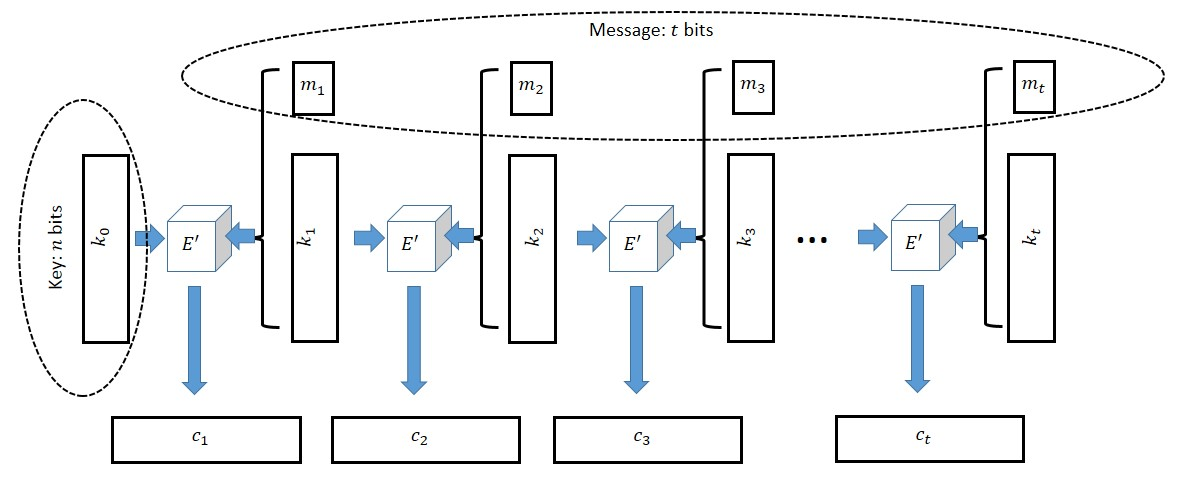
\includegraphics[width=\textwidth, height=0.25\paperheight, keepaspectratio]{../figure/length-extension.jpg}
\caption{Constructing a cipher with \(t\) bit long messages from one
with \(n+1\) long messages}
\label{tmplabelfig}
\end{figure}

\begin{proof} \label[proof]{Let-ttn-We-are-given-a-ci}

Let \(t=t(n)\). We are given a cipher \(E'\) which can encrypt
\(n+1\)-bit long messages with an \(n\)-bit long key and we need to
encrypt a \(t\)-bit long message \(m=(m_1,\ldots,m_t) \in {\{0,1\}}^t\).
Our idea is simple (at least in hindsight). Let
\(k_0 {\leftarrow_{\tiny R}}{\{0,1\}}^n\) be our key (which is chosen at
random). To encrypt \(m\) using \(k_0\), the encryption function will
choose \(t\) random strings
\(k_1,\ldots, k_t {\leftarrow_{\tiny R}}{\{0,1\}}^n\). We will then
encrypt the \(n+1\)-bit long message \((k_1,m_1)\) with the key \(k_0\)
to obtain the ciphertext \(c_1\), then encrypt the \(n+1\)-bit long
message \((k_2,m_2)\) with the key \(k_1\) to obtain the ciphertext
\(c_2\), and so on and so forth until we encrypt the message
\((k_t,m_t)\) with the key \(k_{t-1}\).\footnote{The keys
  \(k_1,\ldots,k_t\) are sometimes known as \emph{ephemeral keys} in the
  crypto literature, since they are created only for the purposes of
  this particular interaction.} We output \((c_1,\ldots,c_t)\) as the
final ciphertext.\footnote{The astute reader might note that the key
  \(k_t\) is actually not used anywhere in the encryption nor decryption
  and hence we could encrypt \(n\) more bits of the message instead in
  this final round. We used the current description for the sake of
  symmetry and simplicity of exposition.}

To decrypt \((c_1,\ldots,c_t)\) using the key \(k_0\), first decrypt
\(c_1\) to learn \((k_1,m_1)\), then use \(k_1\) to decrypt \(c_2\) to
learn \((k_2,m_2)\), and so on until we use \(k_{t-1}\) to decrypt
\(c_t\) and learn \((k_t,m_t)\). Finally we can simply output
\((m_1,\ldots,m_t)\).

The above are clearly valid encryption and decryption algorithms, and
hence the real question becomes \emph{is it secure??}. The intuition is
that \(c_1\) hides all information about \((k_1,m_1)\) and so in
particular the first bit of the message is encrypted securely, and
\(k_1\) still can be treated as an unknown random string even to an
adversary that saw \(c_1\). Thus, we can think of \(k_1\) as a random
secret key for the encryption \(c_2\), and hence the second bit of the
message is encrypted securely, and so on and so forth.

Our discussion above looks like a reasonable intuitive argument, but to
make sure it's true we need to give an actual proof. Let
\(m,m' \in {\{0,1\}}^t\) be two messages. We need to show that
\(E_{U_n}(m) \approx E_{U_n}(m')\). The heart of the proof will be the
following claim:

\textbf{Claim:} Let \(\hat{E}\) be the algorithm that on input a message
\(m\) and key \(k_0\) works like \(E\) except that its the \(i^{th}\)
block contains \(E'_{k_{i-1}}(k'_i,m_i)\) where \(k'_i\) is a
\emph{random} string in \({\{0,1\}}^n\), that is chosen
\emph{independently} of everything else including the key \(k_i\). Then,
for every message \(m\in{\{0,1\}}^t\)

\[
E_{U_n}(m) \approx \hat{E}_{U_n}(m)  \label{lengthextendclaimeq} \;.
\]

Note that \(\hat{E}\) is not a valid encryption scheme since it's not at
all clear there is a decryption algorithm for it. It is just an
hypothetical tool we use for the proof. Since both \(E\) and \(\hat{E}\)
are randomized encryption schemes (with \(E\) using \((t-1)n\) bits of
randomness for the ephemeral keys \(k_1,\ldots,k_{t-1}\) and \(\hat{E}\)
using \((2t-1)n\) bits of randomness for the ephemeral keys
\(k_1,\ldots,k_t,k'_2,\ldots,k'_t\)), we can also write
\eqref{lengthextendclaimeq} as \[
E_{U_n}(m; U'_{tn}) \approx \hat{E}_{U_n}(m; U'_{(2t-1)n})  
\] where we use \(U'_\ell\) to denote a random variable that is chosen
uniformly at random from \(\{0,1\}^\ell\) and independently from the
choice of \(U_n\) (which is chosen uniformly at random from
\(\{0,1\}^n\)).

Once we prove the claim then we are done since we know that for every
pair of message \(m,m'\), \(E_{U_n}(m) \approx \hat{E}_{U_n}(m)\) and
\(E_{U_n}(m') \approx \hat{E}_{U_n}(m')\) but
\(\hat{E}_{U_n}(m) \approx \hat{E}_{U_n}(m')\) since \(\hat{E}\) is
essentially the same as the \(t\)-times repetition scheme we analyzed
above. Thus by the triangle inequality we can conclude that
\(E_{U_n}(m) \approx E_{U_n}(m')\) as we desired.

\textbf{Proof of claim:} We prove the claim by the hybrid method. For
\(j\in \{0,\ldots, \ell\}\), let \(H_j\) be the distribution of
ciphertexts where in the first \(j\) blocks we act like \(\hat{E}\) and
in the last \(t-j\) blocks we act like \(E\). That is, we choose
\(k_0,\ldots,k_t,k'_1,\ldots,k'_t\) independently at random from \(U_n\)
and the \(i^{th}\) block of \(H_j\) is equal to
\(E'_{k_{i-1}}(k_i,m_i)\) if \(i>j\) and is equal to
\(E'_{k_{i-1}}(k'_i,m_i)\) if \(i\leq j\). Clearly,
\(H_t = \hat{E}_{U_n}(m)\) and \(H_0 = E_{U_n}(m)\) and so it suffices
to prove that for every \(j\), \(H_j \approx H_{j+1}\). Indeed, let
\(j \in \{0,\ldots,\ell\}\) and suppose towards the sake of
contradiction that there exists an efficient \(Eve'\) such that

\[
\left| {\mathbb{E}}[ Eve'(H_j)] - {\mathbb{E}}[ Eve'(H_{j+1})]\right|\geq \epsilon \;\;(*)
\]

where \(\epsilon = \epsilon(n)\) is noticeable. By the averaging
principle, there exists some fixed choice for
\(k'_1,\ldots,k'_t,k_0,\ldots,k_{j-2},k_j,\ldots,k_t\) such that \((*)\)
still holds. Note that in this case the only randomness is the choice of
\(k_{j-1}{\leftarrow_{\tiny R}}U_n\) and moreover the first \(j-1\)
blocks and the last \(t-j\) blocks of \(H_j\) and \(H_{j+1}\) would be
identical and we can denote them by \(\alpha\) and \(\beta\)
respectively and hence write \((*)\) as

\[
\left| {\mathbb{E}}_{k_{j-1}}[ Eve'(\alpha,E'_{k_{j-1}}(k_{j},m_j),\beta) - Eve'(\alpha,E'_{k_{j-1}}(k'_j,m_j),\beta) ] \right| \geq \epsilon \;\;(**)
\]

But now consider the adversary \(Eve\) that is defined as
\(Eve(c) = Eve'(\alpha,c,\beta)\). Then \(Eve\) is also efficient and by
\((**)\) it can distinguish between \(E'_{U_n}(k_j,m_j)\) and
\(E'_{U_n}(k'_j,m_j)\) thus contradicting the security of \((E',D')\).
This concludes the proof of the claim and hence the theorem.

\end{proof}

\subsection{Appendix: The computational
model}\label{Appendix-The-computationa}

For concreteness sake let us give a precise definition of what it means
for a function or probabilistic process \(f\) mapping \(\{0,1\}^n\) to
\(\{0,1\}^m\) to be computable using \(T\) operations.

\begin{itemize}
\item
  If you have taken any course on computational complexity (such as
  Harvard CS 121), then this is the model of Boolean circuits, except
  that we also allow randomization.
\item
  If you have not taken such a course, you might simple take it on faith
  that it is possible to model what it means for an algorithm to be able
  to map an input \(x\) into an output \(f(x)\) using \(T\) ``elementary
  operations''.
\end{itemize}

In both cases you might want to skip this appendix and only return to it
if you find something confusing..

The model we use is a Boolean circuit that also has a
\(\ensuremath{\mathit{RAND}}\) gate that outputs a random bit. We could
use as the basic set of gates the standard
\(\ensuremath{\mathit{AND}}\), \(\ensuremath{\mathit{OR}}\) and
\(\ensuremath{\mathit{NOT}}\) but for simplicity we use the one-element
set \(\ensuremath{\mathit{NAND}}\). We represent the circuit as a
straightline program, but this is of course just a matter of
convenience. As shown (for example) in the \href{http://introtcs.org}{CS
121 textbook}, these two representations are identical.

\hypertarget{randprogdef}{}
\begin{definition}[Probabilistic straightline program] \label[definition]{randprogdef}

A \emph{probabilistic straightline program} consists of a sequence of
lines, each one of them one of the following forms:

\begin{itemize}
\item
  \texttt{foo = bar NAND baz} where
  \texttt{foo},\texttt{bar},\texttt{baz} are variable identifiers.
\item
  \texttt{foo = RAND} where \texttt{foo} is a variable identifier.
\end{itemize}

\end{definition}

Given a program \(\pi\), we say that its \emph{size} is the number of
lines it contains. Variables of the form \texttt{X[}\(i\)\texttt{]} or
\texttt{Y[}\(j\)\texttt{]} are considered input and output variables
respectively. If the input variables range from \(0\) to \(n-1\) and the
output variables range from \(0\) to \(m-1\) then the program computes
the probabilistic process that maps \(\{0,1\}^n\) to \(\{0,1\}^m\) in
the natural way. If \(F\) is a (probabilistic or deterministic) map of
\(\{0,1\}^n\) to \(\{0,1\}^m\), the \emph{complexity} of \(F\) is the
size of the smallest program \(P\) that computes it.

If you haven't taken a class such as CS121 before, you might wonder how
such a simple model captures complicated programs that use loops,
conditionals, and more complex data types than simply a bit in
\(\{0,1\}\), not to mention some special purpose crypto-breaking devices
that might involve tailor-made hardware. It turns out that it does (for
the same reason we can compile complicated programming languages to run
on silicon chips with a very limited instruction set). In fact, as far
as we know, this model can capture even computations that happen in
nature, whether it's in a bee colony or the human brain (which contains
about \(10^{10}\) neurons, so should in principle be simulatable by a
program that has up to a few order of magnitudes of the same number of
lines). Crucially, for cryptography, we care about such programs not
because we want to actually run them, but because we want to argue about
their \emph{non existence}.\footnote{An interesting potential exception
  to this principle that every natural process should be simulatable by
  a straightline program of comparable complexity are processes where
  the quantum mechanical notions of \emph{interference} and
  \emph{entanglement} play a significant role. We will talk about this
  notion of \emph{quantum computing} towards the end of the course,
  though note that much of what we say does not really change when we
  add quantum into the picture. As discussed in
  \href{http://introtcs.org}{my lecture notes}, we can still capture
  these processes by straightline programs (that now have somewhat more
  complex form), and so most of what we'll do just carries over in the
  same way to the quantum realm as long as we are fine with conjecturing
  the strong form of the cipher conjecture, namely that the cipher is
  infeasible to break even for quantum computers. (All current evidence
  points toward this strong form being true as well.)} If we have a
process that cannot be computed by a straightline program of length
shorter than \(2^{128}>10^{38}\) then it seems safe to say that a
computer the size of the human brain (or even all the human and nonhuman
brains on this planet) will not be able to perform it either.

\begin{quote}
\textbf{Advanced note:} The computational model we use in this class is
\emph{non uniform} (corresponding to Boolean circuits) as opposed to
\emph{uniform} (corresponding to Turing machines). If this distinction
doesn't mean anything to you, you can ignore it as it won't play a
significant role in what we do next. It basically means that we do allow
our programs to have hardwired constants of \(poly(n)\) bits where \(n\)
is the input/key length. In fact, to be precise, we will hold ourselves
to a higher standard than our adversary, in the sense that we require
our algorithms to be efficient in the stronger sense of being computable
in uniform probabilistic polynomial time (for some fixed polynomial,
often \(O(n)\) or \(O(n^2\))), while the adversary is allowed to use non
uniformity.
\end{quote}
